\newcommand{\sampleheight}{42pt}
\newcommand{\covheight}{46pt}
\newcommand{\marginalheight}{50pt}
\setlength{\tabcolsep}{4pt}
\begin{figure}[t]
  \centering
  \hspace{-1.2em}
  \scalebox{0.9}{
  \begin{centering}
    \begin{tabular}{p{51pt}
      @{\hspace{10pt}}m{2pt}l
      @{\hspace{5pt}}l
      @{\hspace{10pt}}m{2pt}l
      @{\hspace{10pt}}m{2pt}l}
        \raisebox{18pt}{\small$\texttt{Ising}$} &
        \raisebox{34pt}{\rotatebox{90}{\tiny input value}} &
        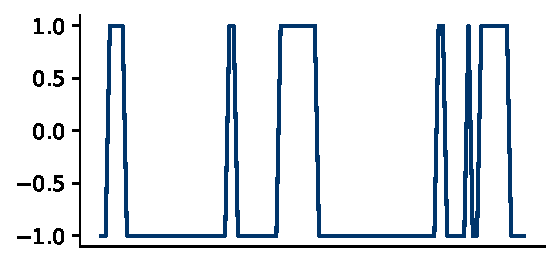
\includegraphics[height=\sampleheight]{figures/task/samples_long/ising.pdf} &
        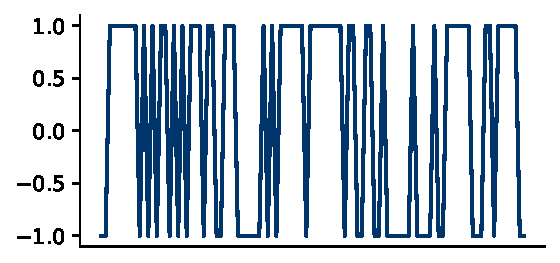
\includegraphics[height=\sampleheight]{figures/task/samples_short/ising.pdf} &
        \raisebox{38pt}{\rotatebox{90}{\tiny input dimension}} &
        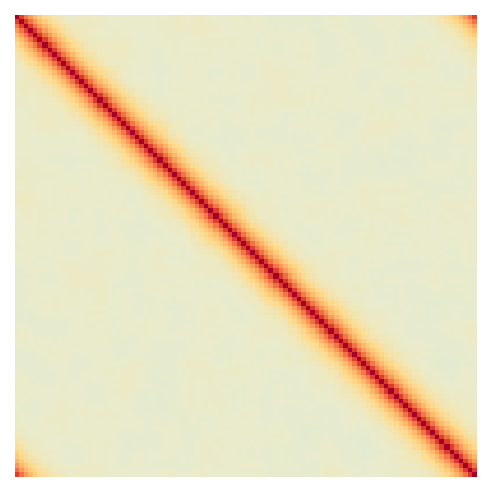
\includegraphics[height=\covheight]{figures/task/cov/ising.pdf} &
        \raisebox{40pt}{\rotatebox{90}{\tiny $p(X_i)$}} &
        \raisebox{-4pt}{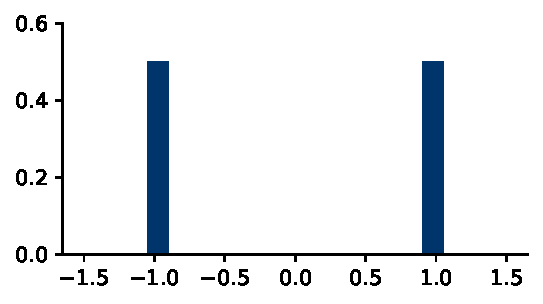
\includegraphics[height=\marginalheight]{figures/task/marginal/ising.pdf}} \\
        \noalign{\vskip -36pt}
        \raisebox{18pt}{\small$\texttt{NLGP}(0.01)$} &
        \raisebox{34pt}{\rotatebox{90}{\tiny input value}} &
        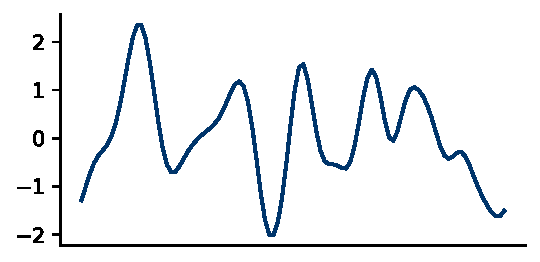
\includegraphics[height=\sampleheight]{figures/task/samples_long/gaussian.pdf} &
        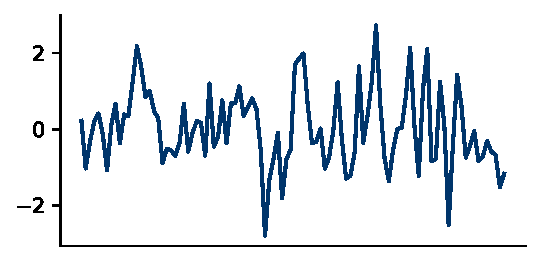
\includegraphics[height=\sampleheight]{figures/task/samples_short/gaussian.pdf} &
        \raisebox{38pt}{\rotatebox{90}{\tiny input dimension}} &
        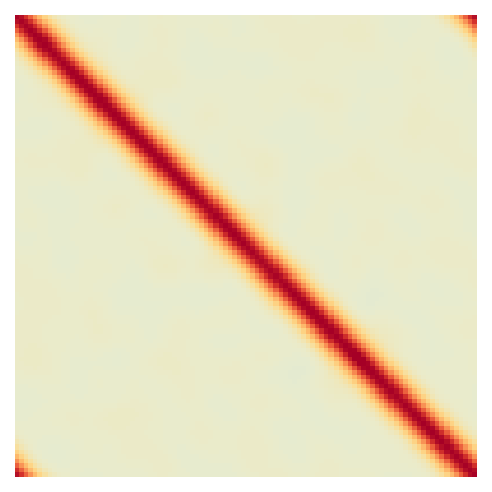
\includegraphics[height=\covheight]{figures/task/cov/gaussian.pdf} & 
        \raisebox{40pt}{\rotatebox{90}{\tiny $p(X_i)$}} &
        \raisebox{-4pt}{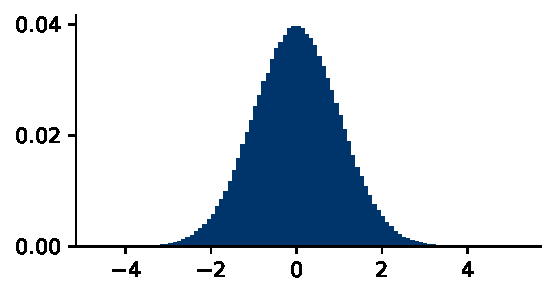
\includegraphics[height=\marginalheight]{figures/task/marginal/gaussian.pdf}} \\
        \noalign{\vskip -36pt}
        \raisebox{18pt}{\small $\texttt{Kur}(5)$} &
        \raisebox{34pt}{\rotatebox{90}{\tiny input value}} &
        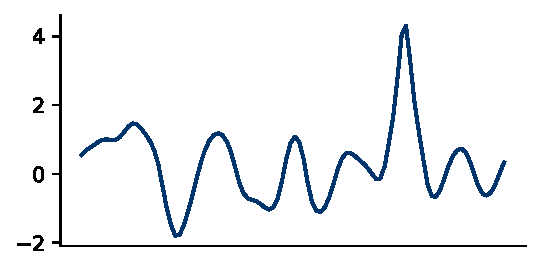
\includegraphics[height=\sampleheight]{figures/task/samples_long/alg5.pdf} &
        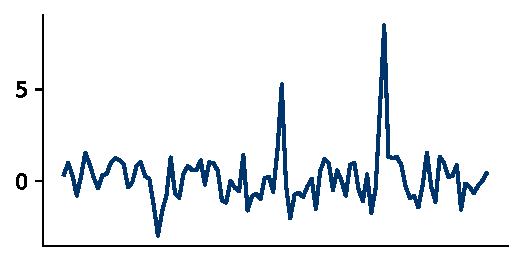
\includegraphics[height=\sampleheight]{figures/task/samples_short/alg5.pdf} &
        \raisebox{38pt}{\rotatebox{90}{\tiny input dimension}} &
        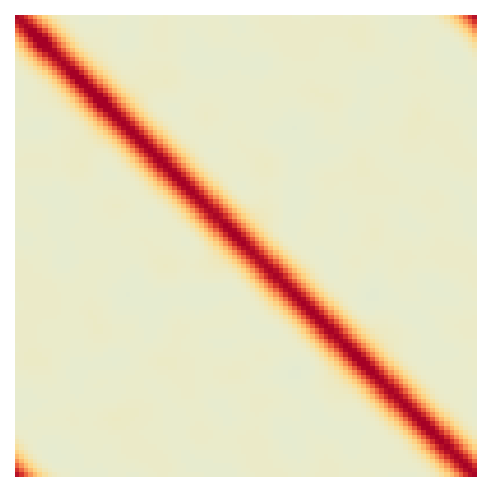
\includegraphics[height=\covheight]{figures/task/cov/alg5.pdf} &
        \raisebox{40pt}{\rotatebox{90}{\tiny $p(X_i)$}} &
        \raisebox{-4pt}{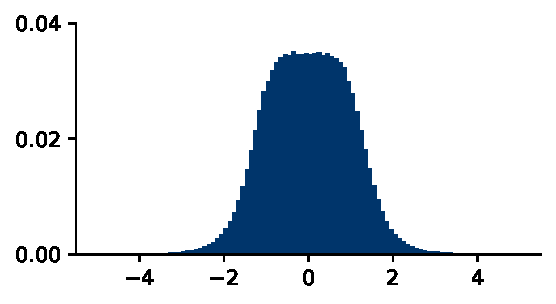
\includegraphics[height=\marginalheight]{figures/task/marginal/alg5.pdf}} \\
        \noalign{\vskip -37pt}
        &&
        \hspace{25pt}\tiny input dimension &
        \hspace{25pt}\tiny input dimension & &
        \hspace{3pt}\tiny input dimension & &
        \hspace{37pt}\tiny input value \\
  \end{tabular}
  \end{centering}
  }
  \caption{
    From left:
    Long- and short-lengthscale samples $\mathbf{x}$,
    covariances $\Sigma$ for one lengthscale,
    and marginals $p(X_i)$ 
    for the data models described in \cref{sec:task}:
    Ising (with $J=1.2, 0.3$ for left, right samples), 
    the nonlinear Gaussian process~\parencite[NLGP;~][]{ingrosso2022data},
    and the controllable kurtosis model, \texttt{Kur}
    (with $\xi=5, 1$ for left, right samples).
    \emph{
    Each model generates samples centered about zero and with covariances that can be constrained to be similar,
    but with differing higher-order statistics, as can be seen from the dimension-wise marginals.
    }
  }
  \label{fig:task}
  \vspace{-10pt}
\end{figure}
